\section{12.6 Metoda Jacobiego}

\begin{frame}{Metoda Jacobiego}
  $$
  A = D + (L+U)
  \begin{cases}
  M=I-D^{-1}A\\
  W=D^{-1}b
  \end{cases}
  $$
  gdzie: L -- poddiagonalna; U -- naddiagonalna;\\
  D = B -- diagonalna, z diagonalnych elementów macierzy A.
  $$Ax = (D+(L+U))x = b \implies Dx = -(L+U)x + b$$
  Korzystając z zależności
  $$\boxed{Dx^{(t+1)}= -(L+U)x^{(t)}+b}$$
  otrzymujemy wzór roboczy:
  $$x_i^{(t+1)}=\frac{1}{a_{ii}}[b_i-\sum_{j=1,j\neq i}^{n} a_{ij}x_j^{(t)}]\  ;\  a_{ii} \neq 0, \forall i \in {1,..,n} $$
\end{frame}
\begin{frame}{Metoda Jocobiego dla równania Poissona}
 \scriptsize{
 $$x_i^{(t+1)}=\frac{1}{a_{ii}}[b_i-\sum_{j=1,j\neq i}^{n} a_{ij}x_j^{(t)}]\  ;\  a_{ii} \neq 0, \forall i \in {1,..,n} $$
  }
  
  \scriptsize{
		    $$
		    \varphi^{(t+1)}(x_i,y_j)=
	 \frac{\rho(x_i,y_j)\cdot h^2 +\varphi^{(t)}(x_{i},y_{j-1})  + \varphi^{(t)}(x_{i-1}, y_j)
	  +\varphi^{(t)}(x_{i+1},y_{j})
	 +\varphi^{(t)}(x_{i},y_{j+1})}{4} 
	 $$
	 }
   \begin{figure}
       \centering
       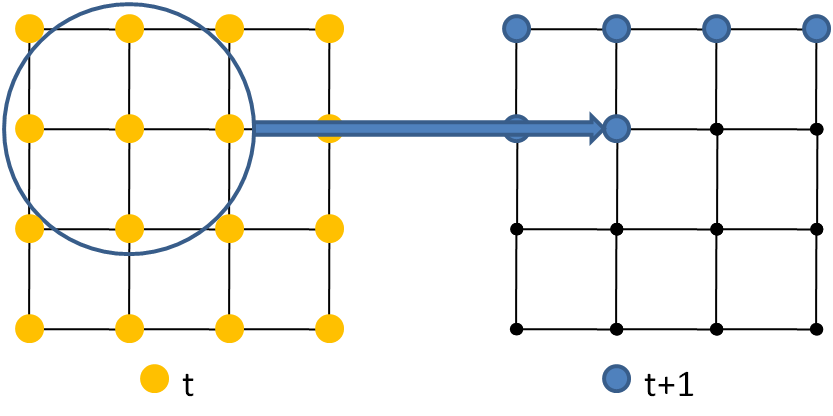
\includegraphics[width=0.8\textwidth]{img/12/jacobi.png}
   \end{figure} 
\end{frame}
\begin{frame}
  \begin{block}{Procedura przestawiania wierszy}
    \begin{itemize}
      \item[1)] spośród kolumn z $a_{ii} = 0$ wybieramy tę, która ma najwięcej zer,
      \item[2)] w tej kolumnie wybieramy element o max $|a_{ji}|$ i przestawiamy wiersze tak, aby znalazł się on na diagonali,
      \item[3)] powtarzamy 1) i 2).
    \end{itemize}
  \end{block}
\end{frame}

\begin{frame}{}
  \begin{block}{Modelowe zadanie}
    równanie Poissona
    \\2-D
    \\warunki brzegowe $\Rightarrow\varphi\equiv 0$
    \\siatka przestrzenna \emph{N x N}
  \end{block}

  \begin{block}{Dla modelowego zadania -- met. Jacobiego:}
    $$\lambda _J=\rho(M_J) = cos\frac{\pi}{N}$$
    $$R_J=log_{10}(cos\frac{\pi}{N})\approx 0.23 (\frac{\pi^2}{N^2})
    $$
    Im większe N tym metoda wolniej zbieżna !
  \end{block}
\end{frame}

\begin{frame}{}
  \begin{block}{Charakterystyka metody Jacobiego}
    \begin{itemize}
      \item prosta,
      \item ma znaczenie dydaktyczne,
      \item wolnozbieżna,
      \item nie wykorzystuje całej, dostępnej w danym kroku informacji,
      \item pamiętane $x^{(t)}$ i $x^{(t+1)}$,
      \item zbieżna dla A silnie diagonalnie dominujących,
      $$\text{wierszowo : }|a_{ii}| > \sum_{j=1,j\neq i}^{n} |a_{ij}|,$$
      $$\text{kolumnowo : }|a_{ii}| > \sum_{j=1,j\neq i}^{n} |a_{ji}|,$$
    \end{itemize}
  \end{block}
\end{frame}
